\chapter{Lower and Upper Bounds}

\chapter{Recycling Gr\o nlund and Pettie's Algorithm}

\section{The Problem}

Given three sets of \(N\) real numbers
\(A = \{\, a_1 < a_2 < \cdots < a_N\,\} \),
\(B = \{\, b_1 < b_2 < \cdots < b_N\,\} \),
and \(C = \{\, c_1 < c_2 < \cdots < c_N\,\}\),
we wish to build a discrete data structure (using bits, words, and pointers) such that,
given any triple \((i,j,k) \in {[N]}^3\) it is possible to compute the sign of
\(a_i + b_j + c_k\) by only inspecting the data structure (we cannot consult
\(A\), \(B\), or \(C\)).
We refer to the map $\chi : {[N]}^3\to \{-,0,+\}, (i,j,k)\mapsto\mathrm{sgn}
(a_i+b_i+c_k)$ as the {\em 3SUM-type} of the instance $\langle A,B,C \rangle$.
Obviously, one can simply construct a lookup table of size \(O(N^3)\), such
that triple queries can be answered in \(O(1)\) time. We aim at improving on
this trivial solution.

\section{Motivation}

In the 3SUM problem, we are given an array of numbers as input and are asked
whether any three of them sum to 0. In the mid-nineties, this problem was
identified as a bottleneck of many
important problems in geometry, such as detection of affine degeneracies or
motion planning~\cite{GO95}. Since then, it has become a central problem in
fine-grained complexity theory~\cite{PW10}. It has long been conjectured to
require $\Omega (N^2)$ time. In 2014, it was shown to be solvable in $o(N^2)$
time, but no algorithm with running time $O(N^{2-\delta})$ with constant
$\delta>0$ is known~\cite{GP18}.

Lower bounds exist in restricted models of computation. Most notably,
$\Omega(N^2)$ 3-linear queries are needed to solve 3SUM~\cite{Er99},
and nontrivial lower bounds have also been proven for slightly more powerful linear
decision trees~\cite{AC05}. However, in a recent breakthrough contribution, Kane, Lovett,
and Moran showed that 3SUM could be solved using $O(N\log^2 N)$
6-linear queries~\cite{KLM18}, hence within a $O(\log N)$ factor of the
information-theoretic lower bound.

Linear decision trees are examples of {\em nonuniform algorithms}, in which we
are allowed to have different algorithms for different input sizes.
Algebraic decision trees generalize linear decision trees
by allowing decision based on the sign of constant-degree polynomials at each
node~\cite{SY82}.

Any decision tree identifying the 3SUM-type of a 3SUM instance yields a concise
encoding of this 3SUM-type:
just write down the outcome of the successive tests. Knowing the decision tree
by convention, this sequence of bits is
sufficient to recover the sign of any triple.

The question we consider here is how to make such a representation efficient,
in the sense that not only does it use merely a few bits, but the answer to any
triple query can be recovered efficiently. Understanding the interplay between
nonuniform algorithms and such data structures hopefully sheds light on the
intrinsic structure of the problem.

\section{Results}

See Table~\ref{tor} for a summary. As there are only $O(N^3)$ queries, a table
of size $(\log_2 3) N^3 + O(1)$ bits suffices to give constant query time
\cite{DPT10}. This can be improved to $O(N^2\log N)$ bits of space by 
storing for each pair $(i,j)$ the values
\(k_<(i,j) = \max \{ 0\}\cup \{k \colon\, a_i + b_j + c_k < 0\}\) and
\(k_>(i,j) = \min \{ N+1\}\cup \{k \colon\, a_i + b_j + c_k > 0\}\).
For a query \((i,j,k)\), we compare \(k\) against the values \(k_<(i,j)\) and \(k_>(i,j)\)
to recover \(\chi(i,j,k)\) in \(O(1)\) time. All \(k_<(i,j)\) and \(k_>(i,j)\)
can be computed in \(O(N^2)\) time via the classic quadratic time algorithm for
3SUM.
%: if \(k \leq k_<(i,j)\), then \(\chi(i,j,k)=-1\), if \( k_<(i,j)< k < k_>(i,j)\),
%then \(\chi(i,j,k)=0\), and if \( k_>(i,j)\leq k\), then \(\chi(i,j,k)=+1\).
%The representation takes \( O(N^2 \log N \) bits, and each query can be answered by comparing
%pairs of indices, which takes \(O(1)\) time.

One seemingly simple representation is to store the numbers in $A$, $B$ and
$C$; however these are reals and thus we need to make them representable using
a finite number of bits.
In Section~\ref{s:numbers} we show that a minimal integer representation of a
3SUM instance may require $\Theta(N)$ bits per value, which would give
rise to a $O(N)$ query time and $O(N^2)$ space, which is far from
impressive.
In \cite{CCILO18} the problem of given a set of $N$ lines, to create an
encoding of them so that the orientation of any triple (the \emph{order type})
can be determined was studied; our problem is a special case of this where the
lines only have three slopes.
Can we do better for the case of 3SUM? We answer this in the affirmative.
In Section~\ref{s:space} we show how to use an optimal $O(N \log N)$ bits of
space with a polynomial query time. Finally, in section~\ref{s:sscqt} we show
how to use $\tilde{O}(N^{1.5})$ space to achieve $O(1)$-time queries.

\begin{table}
\centering
\caption{Table of results}\label{tor}
\begin{tabular}{cccc}
& Query time & Space (in bits) & Preprocessing time \\ \hline
Trivial & $O(1)$ & $O(N^3)$ & $O(N^3)$ \\
Almost trivial & $O(1)$ & $O(N^2 \log N)$ & $O(N^2)$ \\
Order-type encoding \cite{CCILO18} & $O(\log N)$ & $O(\frac{N^2 \log^2 \log N}{\log N})$ & $O(N^2) $\\
Order-type encoding \cite{CCILO18} & $O(\frac{\log N}{\log \log N})$ & $O(\frac{N^2 }{\log^{1-\epsilon} N})$ & $O(N^2)$ \\
Numeric representation (\S\ref{s:numbers}) & $O(N)$ & $O(N^2)$ & $N^{O(1)}$\\
Space-optimal representation (\S\ref{s:space}) & $N^{O(1)}$ & $O(N \log N)$ & $N^{O(1)}$\\
Query-optimal (\S\ref{s:sscqt}) &  $O(1)$ & $\tilde{O}(N^{1.5})$ & $O(N^{2})$ \\
\end{tabular}
\end{table}

\section{Representation by numbers} \label{s:numbers}

A first natural idea is to encode the real 3SUM instance by \emph{rounding} its numbers to integers.
We show a tight bound of $\Theta (N^2)$ bits for this representation.

\begin{lemma}
  \label{lem:bitsize}
Every 3SUM instance has an equivalent integer instance
where all values have absolute value at most $2^{O(N)}$. Furthermore, there
exists an instance of 3SUM where all equivalent integer instances
require numbers at least as large as the $N$th Fibonacci number and where the
standard binary representation of the instance requires $\Omega(N^2)$ bits.
\end{lemma}

\begin{proof}
Every 3SUM instance \(A = \{\, a_1 < a_2 < \ldots < a_N\,\} \), 
\(B = \{\, b_1 < b_2 < \cdots < b_N\,\} \),
and \(C = \{\, c_1 < c_2 < \cdots < c_N\,\}\)
can be interpreted as the point 
\( (a_1,\ldots,a_N,b_1,\ldots,b_N,c_1,\ldots,c_N) \)
in \(\mathbb{R}^{3N}\). 
Let us use the variables \(x_1,\ldots,x_N\) to encode the first \(N\) dimensions
of \(\mathbb{R}^{3N}\), \(y_1,\ldots,y_N\) to encode the next \(N\) dimensions,
and \(z_1,\ldots,z_N$ for the remaining dimensions.
Consider the subset of $\mathbb{R}^{3N}$
\[
	\Delta = \{ (x_1,\ldots,x_N,y_1,\ldots,y_N,z_1,\ldots,z_N) \mid
				x_i<x_{i+1}, ~y_j<y_{j+1}, ~ z_k<z_{k+1}~ \forall i,j,k \in [N-1]\}
\]
and the set $\Pi$ of $N^3$ hyperplanes $x_i+y_j+z_k=0$, where $i,j,k\in [N]$. 
Let $\mathcal{A}$ be the arrangement defined
by $\Pi$ \emph{inside $\Delta$}. Instances of 3SUM correspond to points in $\Delta$.
Moreoever, two 3SUM instances have the same 3SUM-type if and only if they are
in the same cell of $\mathcal{A}$. 

Consider an instance $\langle A,B,C \rangle$ and let $\sigma=\sigma(A,B,C)$ 
be the cell of $\mathcal{A}$ that contains it. 
Then $\sigma$ is the cell defined by the inequalities
\begin{align*}
	\forall{i,j,k}\in [N]&:~~~
	\begin{cases}
		x_i+y_j+z_k > 0 & \text{if $\chi(i,j,k)=+1$,}\\
		x_i+y_j+z_k = 0 & \text{if $\chi(i,j,k)=0$,}\\
		x_i+y_j+z_k < 0 & \text{if $\chi(i,j,k)=-1$.}
	\end{cases}\\
	\forall{i,j,k}\in [N-1]&:~~~
		\begin{cases}
		x_i - x_{i+1}<0,\\
		y_j - y_{j+1}<0,\\
		z_k - z_{k+1}<0.
	\end{cases}
\end{align*}
Let $\sigma'$ be the subset of $\mathbb{R}^{3N}$ defined by the following inequalities:
\begin{align*}
	\forall{i,j,k}\in [N]&:~~~
	\begin{cases}
		x_i+y_j+z_k \geq 1 & \text{if $\chi(i,j,k)=+1$,}\\
		x_i+y_j+z_k = 0 & \text{if $\chi(i,j,k)=0$,}\\
		x_i+y_j+z_k \leq -1 & \text{if $\chi(i,j,k)=-1$.}
	\end{cases}\\
	\forall{i,j,k}\in [N-1]&:~~~
		\begin{cases}
		x_i - x_{i+1} \leq 1,\\
		y_j - y_{j+1} \leq 1,\\
		z_k - z_{k+1} \leq 1.
	\end{cases}
\end{align*}

Clearly $\sigma'$ is contained in $\sigma$. Moreover, for a sufficiently large $\lambda>0$
the scaled instance $\langle \lambda A,\lambda B,\lambda C \rangle$ belongs to $\sigma'$.
Therefore, $\sigma'$ is nonempty.

Since $\sigma'$ is defined by a collection of linear inequalities defining closed halfspaces,
there exists a point $p$ in $\sigma'$ defined by a subset of at most $3N$ inequalities, 
where the inequalities are actually equalities. Let us assume for simplicity that
exactly $3N$ equalities define the point $p$. Then, $p=(x,y,z)$ is the solution
to a linear system of equations $M [x~ y ~z]^T=\delta$ 
where $M$ and $\delta$ have their entries in $\{ -1,0,1 \}$
and each row of $M$ has at most three non-zero entries. The solution $p$ to this
system of equations is an instance equivalent to $\langle \lambda A,\lambda B,\lambda C \rangle$.

Because of Cramer's rule, the system of linear equations has solution with entries
$\det(M_i)/\det(M)$,
where $M_i$ is the matrix obtained by replacing the $i$th column of $M$ by $\delta$.
We use the following simple bound on the determinant.
Since $\det(M)=\sum_{\pi}\mathrm{sgn}(\pi) \prod_i m_{i,\pi(i)}$, where
$\pi$ iterates over the permutations of $[3N]$, there are 
at most $3^{3N}$ summands where $\pi$ gives non-zero product $\prod_i m_{i,\pi(i)}$ (we have
to select one non-zero entry per row), and the product is always in $\{ -1,0,1\}$.
Therefore $|\det(M)|\leq 3^{3N}$. Similarly, $|\det(M_i)|\leq 4^{3N}$ because
each row of $M_i$ has at most $4$ non-zero entries.
We conclude that the solution to the system $M [x~ y ~z]^T=\delta$ 
are rationals that can be expressed with $O(N)$ bits. This solution gives
a 3SUM instance with rationals that is equivalent to $\langle A, B, C \rangle$. 
Since all the rationals have the common denominator ($\det(M)$), we can scale the result
by $\det(M)$ and we get an equivalent instance with integers, where 
each integer has $O(N)$ bits.

The proof of the second statement is by implementing the Fibonacci recurrence in each of the
arrays $A,B,C$. This can be achieved by letting:
\begin{eqnarray*}
  a_i + b_1 + c_{N-i+1} & = & 0, \text{for }i\in [N] \\
  a_1 + b_i + c_{N-i+1} & = & 0, \text{for }i\in [N] \\
  a_{i-1} + b_{i-2} + c_{N-i+1} & < & 0, \text{for }i\in \{3,4,\ldots ,N\},
\end{eqnarray*}
The first two sets of equations ensure that the two arrays $A$ and $B$ are identical, while
the array $C$ contains the corresponding negated numbers, in reverse order.
From the inequalities in the third group, and depending on the choice of the initial values $a_1, a_2$,
each array contains a sequence growing at least as fast as the Fibonacci sequence.
\end{proof}

Note that this is a much smaller lower bound than for order types of points sets in the plane,
the explicit representation of which can be shown to require exponentially many bits per coordinate~\cite{GPS89}.

\section{Space-optimal representation} \label{s:space}

By considering the arrangement of hyperplanes defining the 3SUM problem, we get an
information-theoretic lower bound on the number of bits in a 3SUM-type.

\begin{lemma}
  There are $2^{\Theta(N\log N)}$ distinct 3SUM-types of size $N$.
\end{lemma}
\begin{proof}
  3SUM-types of size $N$ are in one-to-one correspondence with cells of the
  arrangement of $N^3$ hyperplanes in $\mathbb{R}^{3N}$. The
  number of such cells is $O(N^{9N})$ and at least ${(N!)}^2$.
\end{proof}

In order to reach this lower bound, we can simply
encode the label of the cell of the arrangement in \(\Theta(N \log N)\) bits.
However, decoding the information
requires to construct the whole arrangement which takes \(N^{O(N)}\) time.
An alternative solution is to store a
vertex of the arrangement of hyperplanes \(a_i + b_j + c_k \in \{\,
-1, 0, 1\,\}\).
There exists such a vertex that has the same 3SUM-type as the input point, as shown in the proof of Lemma~\ref{lem:bitsize}.
To answer any query, either recompute the vertex from the basis then answer the query using arithmetic,
or use linear programming. 
Hence we can build a data structure of $O(N\log N)$ bits such that triple queries can be answered in polynomial time.

Note that we do not exploit much of the 3SUM structure here. In particular, the
same essentially holds for $k$-SUM, and can also be generalized to a {\sc
Subset Sum} data structure of $O(N^2)$ bits, from which we can extract the sign
of the sum of any subset of numbers.

\section{Subquadratic space and constant query time}\label{s:sscqt}
Our encoding is inspired by  Gr{\o}nlund and Pettie's $\tilde{O}(N^{1.5})$
non-uniform algorithm for 3SUM~\cite{GP18}.
Our data structure stores three components, which we call the
\emph{differences}, the \emph{staircase} and the \emph{square neighbors}.

\begin{description}
\item[Differences.]
  Partition $A$ and $B$ into \emph{blocks} of $\sqrt{N}$ consecutive elements.
  Let $D$ be the set of all differences of the form $a_{i_1}-a_{i_2}$ and
  $b_{j_1}-b_{j_2}$
  where the items come from the same block. There are $O(N^{1.5})$ such
  differences. Sort $D$ and store a table indicating for each difference in $D$
  its rank among all differences in $D$. This takes $O(\log N)$ bits for each
  of the $O(N^{1.5})$ differences, for a total of $O(N^{1.5}\log N)$ bits.

\item[Staircase.]
  Look at the table $G$ formed by all sums of the form $a_i+b_j$. It is
  monotonic in its rows and columns due to $A$ and $B$ being sorted. We view it
  as being partitioned into a grid $G'$ of size $\sqrt{N}\times \sqrt{N}$ where
  each \emph{square} of the grid is also of size $\sqrt{N}\times \sqrt{N}$.
  %
  For each element $c_k \in C$, for each $i'\in[1,\sqrt{N}]$ we store the largest
  $j'$ such that some elements of the square $G'[i',j']$ are  $< c$, denote this as
  $L[k,i']$.
  %
  We also store, for each $c_k \in C$, for each $i'\in[1,\sqrt{N}]$ the smallest
  $j'$ such that some elements of the square $G'[i',j']$ are  $\geq c$, denote this as
  $U[k,i']$.
  %
  We thus store, in $L$ and $U$, $2 \sqrt{N}$ values of size $O(\log N)$ for each
  of the $N$ elements of $C$, for a total space usage of $O(N^{1.5}\log N)$ bits.
  %
  We call this the \emph{staircase} as this implicitly classifies, for each $c
  \in C$, whether each square has elements larger than $c$, smaller than $c$, or
  some larger and some smaller; only $O(\sqrt{N})$ can be in the last case, which
  we refer to as the \emph{staircase} of $c$.

\item[Square neighbors.]
  For each element $c_k \in C$, for each of the $O(\sqrt{N})$ squares on the
  staircase, we store the location of the predecessor and successor of $c_k$.
  Those squares are the \(G'[i',j']\) such that
  $L[k,i'] \le j' \le U[k,i']$, for $i',j' \in [1,\sqrt{N}]$.
  This takes space $O(N^{1.5}\log N)$.
\end{description}

To execute a query $(a_i,b_j,c_k)$, only a constant number of lookups in the
tables stored are needed.
Let us define \(i' = \lceil i / \sqrt{N} \rceil\)
and \(j' = \lceil i / \sqrt{N} \rceil\) to be the indices of the cell of
\(G'\) containing the point \((a_i, b_j)\).
If $j' < L[k,i']$, then we know $a_i + b_j < c_k$.
If $j' > U[k,j']$, then we know $a_i + b_j > c_k$.
If neither of these is true, then the square $G'[i',j']$ is on the staircase of
$c_k$ and thus using
the square neighbors table we can determine the location of the predecessor and
successor of $c_k$ in this square; suppose they are at $G[s_i,s_j]$ and
$G[p_i,p_j]$ and thus $G[s_i,s_j] \leq c_k \leq G[p_i,p_j]$. One need only
determine how these two compare to $G[i,j]=a_i+b_j$ to answer the query. But
this can be done using the differences as follows: to compare $G[s_i,s_j]$ to
$G[i,j]$ this would be determining the sign of $(a_i+b_j)-(a_{s_i}+b_{s_j})$
which is equivalent to determining the result of comparing $a_i-a_{s_i}$ and
$b_j-b_{s_j}$, which since both are in the same square, these differences are
in $D$ and the comparison can be obtained by examining their stored ranks. By
doing this for the predecessor and successor we will determine the relationship
between $a_i+b_j$ and $c_k$.

\begin{figure}
\centering
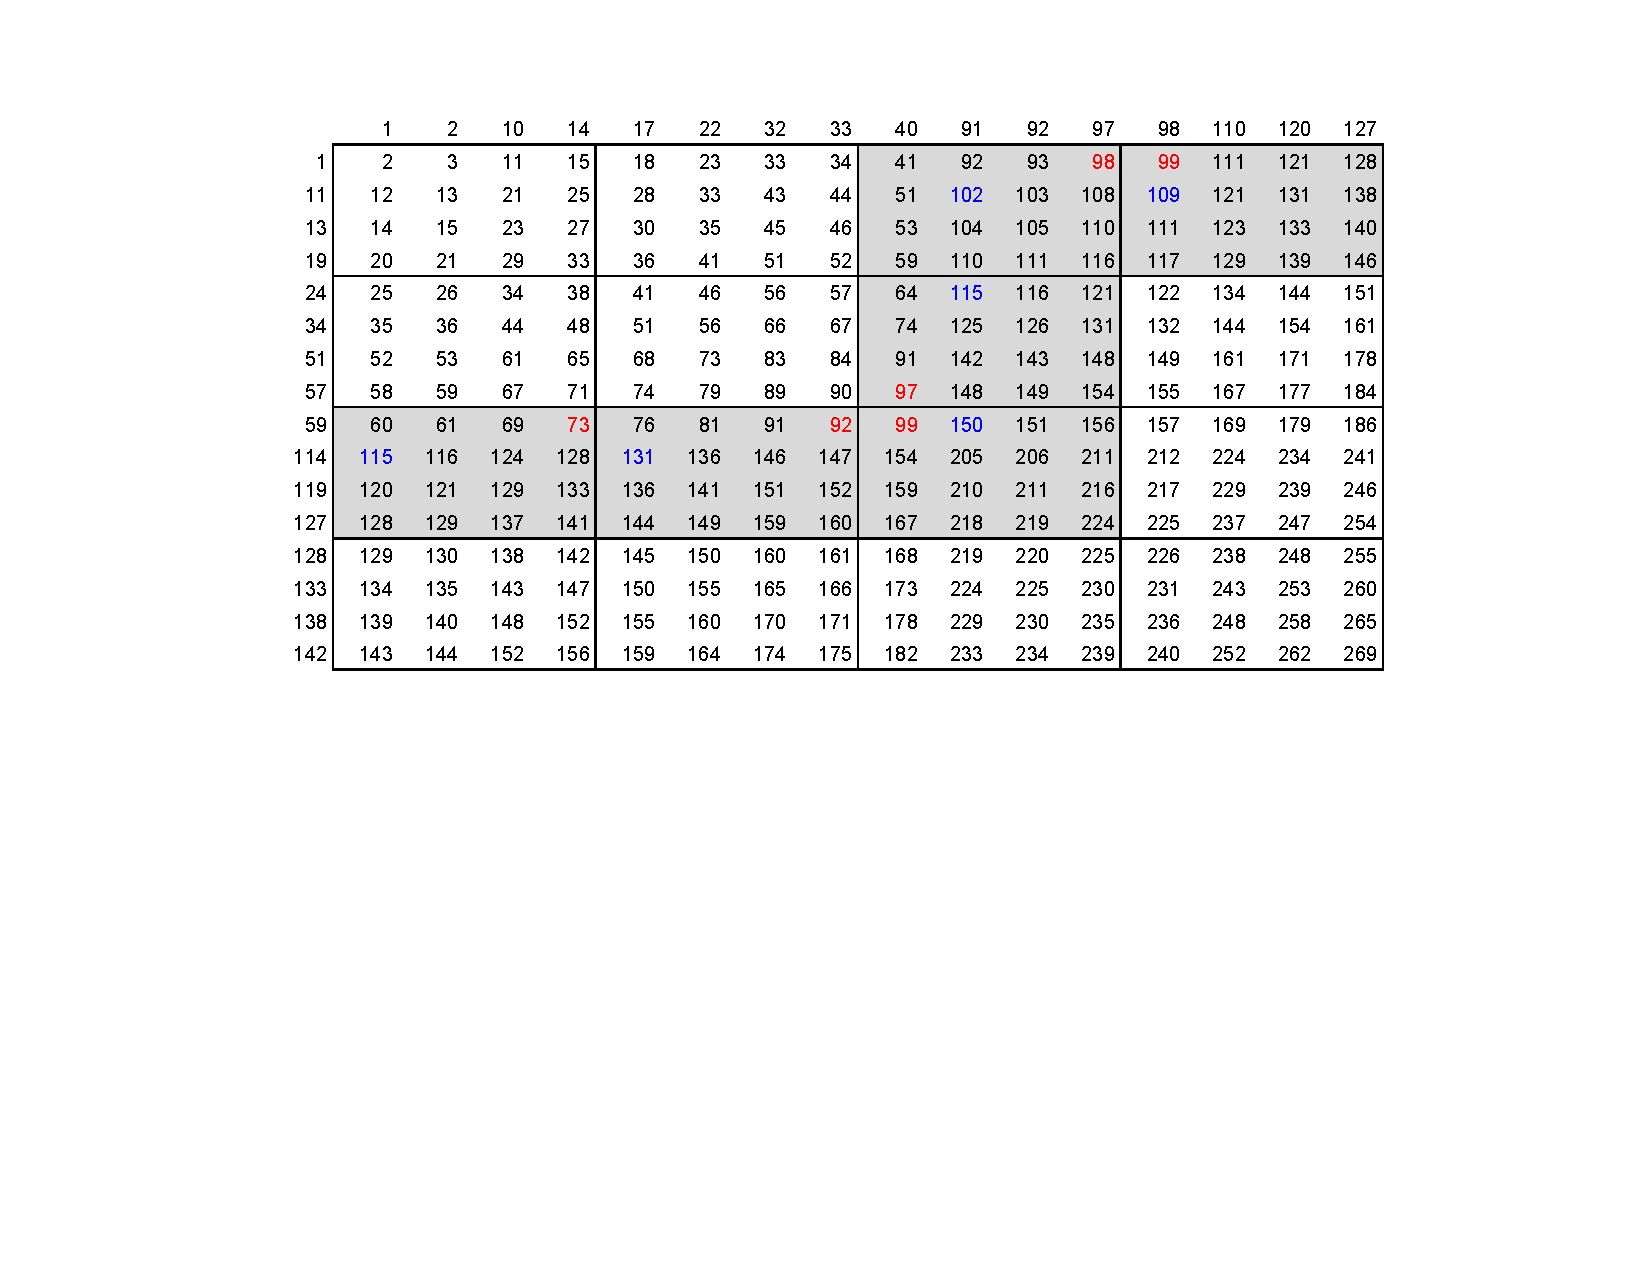
\includegraphics[trim={4cm 10cm 3cm 2cm},clip,width=5.5in]{figures/stair}
\caption{Illustration of the staircase and square neighbors of the constant query time encoding. Here the $16\times16$ table is partitioned into a $4\times 4$ grid of squares of size $4\times 4$. If $c_k=100$, the grey illustrates the squares that form the staircase, containing values both larger and smaller than 100. Predecessors and successors within each staircase square are shown in red and blue.}
\end{figure}

%Because 3SUM reduces to GPT, we can reuse the data structure in~\cite{CCILO18} after reduction.
%Our encoding is based on using Gr{\o}nlund and Pettie's $\tilde{O}(N^{1.5})$ non-uniform algorithm for 3SUM, which we review.
%
%
%
%\begin{enumerate}
%  \item[1] Choose a parameter \(g \leq n\).
%  \item[2] Divide \(A\) and \(B\) into \emph{blocks} \(A_i\) and \(B_j\) of \(g\) consecutive elements.
%  \item[3] For each pair of blocks \((A_i,B_j)\) sort the set \(\{\, a + b
%    \colon\, (a,b) \in A_i \times B_j\,\}
%    \)
%  \item[4] For each \(c \in C\), and each pair \((A_i, B_j)\) such that the line
%    \(x+y=-c\) intersects the set \(\operatorname{conv}(A_i \times B_j)\)
%    binary search for \(-c\) in the set \(A_i \times B_j\).
%\end{enumerate}
%
%Two important observation give this algorithm a (nonuniform) running
%time of \(\tilde{O}(n^{\frac 32})\):
%\begin{itemize}
%  \item[(1)] For step 3, observe that sorting those
%  sets by comparison only involves comparisons of the type \(a + b \leq a' + b'\)
%  where \(a\) and \(a'\) belong to the same block \(A_i\)
%  and \(b\) and \(b'\) belong to the same block \(B_j\). Hence, from a
%  nonuniform point of view, it is sufficient to sort all numbers \(a-a'\) and
%  \(b'-b\) obtained by manipulating those comparisons. There are \(O(\frac ng
%  \cdot
%  g^2 ) = O(ng)\) such pairs, hence sorting them costs \( \tilde{O}(ng) \)
%  time.
%\item[(2)] Because each line \(x+y=-c\) draws a \emph{staircase} in the grid defined
%  by the rectangles \(\operatorname{conv}(A_i \times B_j)\), only \(O(\frac
%  ng)\) rectangles are hit by that line. Hence, the cumulative cost of searching
%  for each \(-c\) in those sets is \( \tilde{O}(n \cdot \frac ng) =
%  \tilde{O}(\frac{n^2}{g})\).
%\end{itemize}
%
%We choose \(g = \Theta(\sqrt{N})\) to balance those two expressions and obtain a
%nonuniform running time of
%\(\tilde{O}(n^{\frac 32})\).
%
%The algorithm presented above already constructs a data structure. We adapt
%it to solve the problem at hand.
%
%Recall that we wish to answer queries of the type \(f(i,j,k) = a_i + b_j + c_k
%<=> 0\).
%
%\subparagraph{Compute the cell \(A_u \times B_v\) containing \((a_i, b_j)\).}
%Let \(u = \lfloor \frac ig \rfloor\) and \(v = \lfloor \frac jg \rfloor\).
%
%\subparagraph{Determine the location of that cell with respect to the staircase defined by
%\(c_k\).}
%We have stored, for each pair \((u,v)\), a \(k^-\) and a \(k^+\) such that
%\(c_{k^-}\) defines the first line entirely below that set and \(c_{k^+}\)
%defines the first line entirely above that set.%
%\footnote{%
%Note that we can use sentinel values for boundary cases. This comment also
%applies later.%
%}
%%
%This costs a total of \(2 \frac{n^2}{g^2} \cdot \log n\) bits and
%allows to test in constant time whether \(c_k\) lies above, below, or intersect
%that set by comparing \(k\) to \(k^-\) and \(k^+\).
%If that set is not on the staircase defined by \(c_k\) then we readily know the
%answer to the query.
%
%\subparagraph{Compare \(a_i + b_j\) to the predecessor and successor of
%\(c_k\) in \(A_u \times B_v\).}
%For each triple \(c_k, A_u, B_v\) where the staircase defined by
%\(c_k\) contains the set \(A_u \times B_v\) we have stored the pairs
%\((i^-,j^-)\) and \((i^+, j^+)\) such that
%\(a_{i^-} + b_{j^-}\) is the largest number in \(A_u + B_v\) strictly smaller than
%\(c_k\)
%and
%\(a_{i^+} + b_{j^+}\) is the smallest number in \(A_u + B_v\) strictly larger than
%\(c_k\). This takes \(4 n \cdot \frac ng \cdot \log g =
%\tilde{O}(\frac{n^2}{g})\) bits total. If we can compare \(a_i + b_j\) to those two
%numbers we obtain the answer to the query.
%
%To be able to compare those numbers in constant time we store for each
%pair \((a_i,a_{i'})\) belonging to the same block \(A_u\), and for each pair
%\((b_j,b_{j'})\) belonging to the same block \(B_v\), their rank in a sorted
%permutation of the union of all \(A_u - A_u\) and \(B_v - B_v\).
%Testing for
%\(a_i + b_j \leq a_{i^-} + b_{j^-}\)
%amounts to testing for
%\(a_i - a_{i^-} \leq b_{j^-} - b_j\) which can be done in constant time given
%those ranks. This takes an extra \( \tilde{O}(ng) \) space.
%
%Like in the GP algo, balancing gives \( \tilde{O}(n^{\frac 32}) \) space. Queries
%take constant time.
%
%\subparagraph*{Acknowledgments.} We thank the organizers for the organization.
